\documentclass{IEEEtran}
\usepackage[spanish]{babel} % Definir el idioma del documento
\usepackage[letterpaper,top = 2cm, bottom = 2cm, left = 2cm, right = 2cm, marginparwidth = 1.75cm]{geometry} % Especificar los márgenes según la norma
\usepackage{pdfpages} % Añadir PDFs y que te cuente las páginas para el documento
\usepackage{subfiles} % Tener subdocumentos (hay más opciones)
\usepackage{tableof} % Se utiliza para los indices de los subdocumentos
\usepackage{float} % Para usar lo de 'H'
\usepackage{fancyhdr}
\usepackage{comment}
\usepackage{biblatex} % Paquete para manejar citas y bibliografía
\usepackage{amsmath}
\addbibresource{bibliografia.bib} % Cargar el archivo .bib

\def\TituloProyecto{Estudio del Recurso Eólico en Tarifa}
\def\Autor{Mercedes Román Ruiz}
\def\Asignatura{Fuentes de Energía}
\def\Curso{2024 - 25}
\def\Fecha{Diciembre 2024}

% ---------------------------- LOS TRUQUITOS -------------------------------------------------
% Si se incluye [H] la tabla, grafica o imagen en el sitio en el que se está escribiendo, sin importar las sugerencias de LaTeX
% --------------------------------------------------------------------------------------------

\begin{document}
\sloppy 
\setlength{\parindent}{30pt}
\setlength{\parskip}{6pt}
\renewcommand\thesection{\arabic{section}}
\renewcommand{\baselinestretch}{1.5}
% \renewcommand{\listtablename}{Índice de tablas} % Si no se hace esto, aparece como 'Indice de Cuadros'
% \renewcommand{\tablename}{Tabla} % Si no se hace esto, aparece como 'Cuadro'

\fancyhead{}
\fancyfoot{}
%\pagestyle{fancy}
\chead[\rightmark]{\leftmark}
\fancypagestyle{plain}{%
    \cfoot{ }%
    \renewcommand{\headrulewidth}{0pt}
    \fancyhf{ }%
}

\fancyfoot[LE,RO]{\thepage}

\begin{titlepage}
    \centering
    
\includegraphics[width=0.5\linewidth]{Imagenes/Logo UPM.png} \par
    \vspace{1cm}
    {\bfseries\LARGE Escuela Técnica Superior de Ingenieros Industriales \par}
    \vspace{0.5cm}
    {\scshape\Large Máster en Ingeniería Industrial \par}
    \vspace{3 cm}
    {\itshape\huge Informe Técnico \par}
    \vspace{0.5cm}
    {\Huge \textbf{\TituloProyecto} \par}
    \vfill
    {\Large Autora: Mercedes Román Ruiz \par}
    \vspace{0.5cm}
    %{\Large \Asignatura \  \Curso \par}
    %\vspace{0.5cm}
    {\Large \Fecha \par}
\end{titlepage}

\tableofcontents
% \pagebreak

\section{Introducción}
% Una primera sección denominada "1. Introducción". En dos o tres párrafos se contesta a las preguntas: ¿cuál es el objetivo del informe? y ¿cómo se ha elaborado el informe?

Este informe se enmarca en la asignatura Fuentes de Energía del Máster en Ingeniería Industrial, formando parte de la evaluación continua de la asignatura. Para su desarrollo, se selecciona un emplazamiento a analizar para luego realizar un estudio de la viabilidad de un parque eólico en la ubicación seleccionada.

Para la elaboración de este trabajo se utilizarán los datos reales existentes a lo largo de todo el mundo. Haciendo uso de la base de datos climatológicos de NASA Prediction of Worldwide Energy Resorces \cite{NASA2024}

Se decide estudiar un punto con coordenadas: 36.0014, -5.6096; situado en la Isla de Tarifa, también conocida como Isla de Las Palomas.

\section{Análisis preliminar de los datos de viento}
% Una segunda sección con los resultados del análisis preliminar de los datos de viento en la ubicación seleccionada. "2. Análisis preliminar de los datos de viento". Esta sección incluirá el análisis preliminar de los datos eólicos discutiendo su calidad.

% ----------------------------------------------------------------------------------------------

% Describir las magnitudes de interés, sus unidadees y la frecuencia de muestreo

En el estudio eólico se va a trabajar con las velocidades del viento y su dirección, medidas a $10\ m$. Dichos datos fueron muestreados cada hora, y tienen unidades de $m/s$ y $^\circ$ respectivamente.

% Evaluar cuantitativamente la cantidad de datos erróneos para cada año del periodo seleccionado

Con el objetivo de tener una muestra significativa se va a analizar un periodo de 4 años, abarcando desde el 1 de Enero de 2020 hasta el 31 de Diciembre de 2023. Tal y como se indica en la base de datos utilizada, aquellos datos que por error cometido o falta de medición no se encuentren tendrán un valor de `-999'.

Cabe destacar que el año 2020 fue un año bisiesto y por ende tuvo 366 días, con lo que cuenta con 24 mediciones más en comparación con los otros años que abarca el estudio.

% Discutir la calidad de los datos e indicar que periodos son relevantes para el estudio eólico de la ubicación. Seleccionar el año más reciente que tenga una buena calidad de datos.

Esta base de datos no muestra información sobre la calidad de las mediciones por lo que se suponen que estos son válidos. Se decide utilizar como año representativo el año 2023.


\section{Estudio estadístico del recurso eólico en la ubicación}
% Después una sección con el estudio estadístico del recurso eólico. "3. Estudio estadístico del recurso eólico en la ubicación". El análisis se competará con las figuras más relevantes que se mencionan en la rúbrica. Cada figura debe ser descrita en el texto y acompañada de una pequeña discusión sobre el resultado.

% ----------------------------------------------------------------------------------------------

\subsection{Análisis estadístico anual}
% Análisis estadístico anual de los datos recopilados en los últimos 4 años con momentos estadísticos (velocidad media y varianza). Para ello se evalúan los momentos estadísticos por año, y se representará en una gráfica la media y varianza en función del año.

Se comienza con un análisis anual de los datos recopilados, representando en la figura \ref{fig: Analisis estadistico anual} la velocidad media y varianza de cada año de la tabla \ref{tab: Velocidad media y varianza por año}.

\begin{table}[h]
    \centering
    \label{tab: Velocidad media y varianza por año}
    \caption{Velocidad media y varianza por año.}
    \begin{tabular}{|c|c|c|}
        \hline
        Años & Velocidad \textsubscript{media} (m/s) & Varianza (m/s) \\
        \hline
        2020 & 4.5670 & 5.8953 \\
        2021 & 4.7042 & 6.5410 \\
        2022 & 4.7081 & 6.8754 \\
        2023 & 4.5046 & 6.1034 \\
        \hline
    \end{tabular}
\end{table}

\begin{figure}[h]
    \centering
    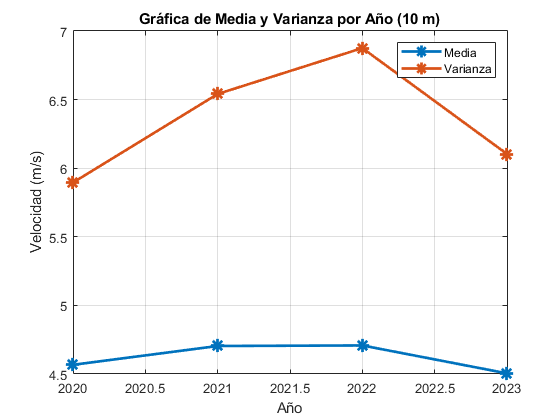
\includegraphics[width = 0.5 \textwidth]{Imagenes/Grafica de Media y Varianza por Año.png}
    \caption{Análisis estadístico anual.}
    \label{fig: Analisis estadistico anual}
\end{figure}

La velocidad media se mantiene estable con valores entre $[4.5046,\ 4.7081]\ m/s$ en los años estudiados.

\subsection{Análisis estadístico estacional}
% Análisis estadístico estacional de los datos recopilados en los últimos 4 años con momentos estadísticos (velocidad media y varianza). Para ello se evalúan los momentos estadísticos por meses, y se representará en una gráfica la media y varianza en función de los meses.

El análisis estadístico de los datos continua realizando un estudio de la velocidad media y varianza por meses. Dichos resultados se muestran en la tabla \ref{tab: Velocidad media y varianza por mes} y se grafican en la figura \ref{fig: Analisis estadistico mensual}.

\begin{table}[h]
    \centering
    \label{tab: Velocidad media y varianza por mes}
    \caption{Velocidad media y varianza por mes.}
    \begin{tabular}{|c|c|c|}
        \hline
        Mes & Velocidad \textsubscript{media} (m/s) & Varianza (m/s) \\
        \hline
        Enero & 5.1354 & 7.1307 \\
        Febreo & 5.8816 & 9.5316 \\
        Marzo & 4.8047 & 7.9160 \\
        Abril & 4.9397 & 7.5128 \\
        Mayo & 4.3980 & 6.2028 \\
        Junio & 4.1983 & 4.0598 \\
        Julio & 4.2268 & 4.8861 \\
        Agosto & 3.6672 & 3.3029 \\
        Septiembre & 4.0737 & 4.4757 \\
        Octubre & 4.9204 & 6.0305 \\
        Noviembre & 4.4191 & 5.5407 \\
        Diciembre & 4.8705 & 6.3040 \\
        \hline
    \end{tabular}
\end{table}

\begin{figure}[h]
    \centering
    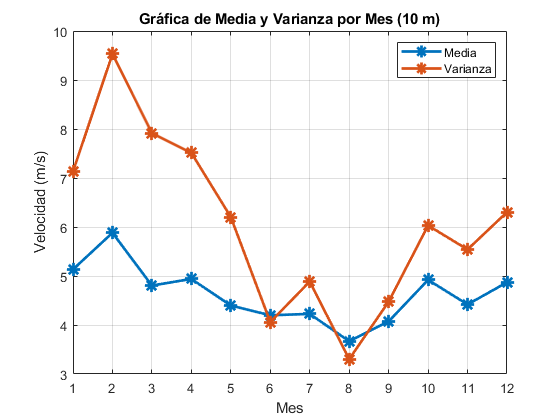
\includegraphics[width = 0.5 \textwidth]{Imagenes/Grafica de Media y Varianza por Mes.png}
    \caption{Análisis estadístico mensual.}
    \label{fig: Analisis estadistico mensual}
\end{figure}

Como se observa en la figura \ref{fig: Analisis estadistico mensual}, tanto la velocidad media como la varianza tienen su máximo en en el mes de Febrero, y su mínimo en Agosto. Haciéndose notar así el cambio de estación de invierno a verano.

\subsection{Análisis estadístico estacional por periodo}
% Análisis estadístico estacional distingueindo periodo diurno y nocturno de los datos recopilados en los últimos 4 años con momentos estadísticos (velocidad media y varianza). Para ello se evalúan los momentos estadísticos por meses, distinguiendo los periodos diurnos (10:00 - 18:00) y nocturnos (22:00 - 06:00), y se representará en una gráfica la media y varianza en función de los meses.
Al análisis estadístico estacional anterior se le añade la distinción entre periodos diurnos (10:00 - 18:00) y nocturnos (22:00 - 06:00). Obteniéndose los resultados de la tabla \ref{tab: Velocidad media y varianza por mes (periodo diurno y nocturno)}.

\begin{table}[h]
    \centering
    \label{tab: Velocidad media y varianza por mes (periodo diurno y nocturno)}
    \caption{Velocidad media y varianza por mes (periodo diurno y nocturno).}
    \begin{tabular}{|c|c|c|c|c|}
        \hline
        & \multicolumn{2}{|c|}{Diurno} & \multicolumn{2}{c|}{Nocturno} \\
        \hline
        Mes & Vel \textsubscript{media} (m/s) & Var (m/s) & Vel \textsubscript{media} (m/s) & Var (m/s) \\
        \hline
        Enero & 5.1926 & 8.1462 & 5.1126 & 6.4542 \\
        Febrero & 6.0618 & 10.6110 & 5.7717 & 8.9609 \\
        Marzo & 5.0250 & 8.9256 & 4.6567 & 6.9644 \\
        Abril & 5.1206 & 8.5657 & 4.7970 & 6.4524 \\
        Mayo & 4.5083 & 7.2615 & 4.3579 & 5.0647 \\
        Junio & 4.5263 & 4.7582 & 3.9345 & 3.2441 \\
        Julio & 4.4471 & 5.8149 &  4.0682 & 3.8732 \\
        Agosto & 3.9314 & 3.9560 & 3.4736 & 2.4707 \\
        Septiembre & 4.3546 & 5.1022 & 3.8745 & 3.8923 \\
        Octubre & 5.2163 & 7.1533 & 4.7171 & 4.9273 \\
        Noviembre & 4.6327 & 6.7886 & 4.2625 & 4.4599 \\
        Diciembre & 5.0049 & 6.9589 & 4.8071 & 6.0037 \\
        \hline 
    \end{tabular}
\end{table}

\begin{figure}[h]
    \centering
    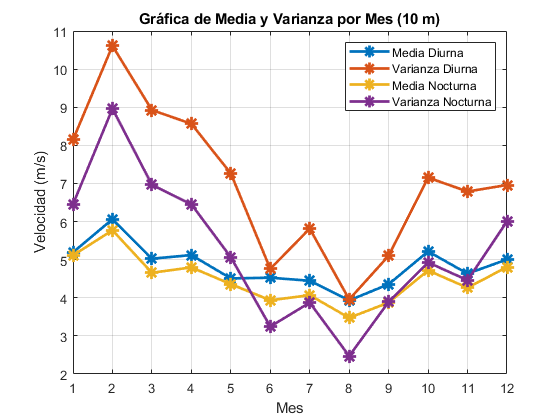
\includegraphics[width = 0.5 \textwidth]{Imagenes/Grafica de Media y Varianza por Mes Periodo Diurno y Nocturno.png}
    \caption{Análisis estadístico mensual por periodo.}
    \label{fig: Analisis estadistico mensual por periodo}
\end{figure}

En la figura \ref{fig: Analisis estadistico mensual por periodo} puede verse que las velocidades medias diurnas y nocturnas mantienen una tendencia general similar, con valores más altos durante los meses de invierno, y con mínimos en los meses de verano. Asimismo, la varianza diurna presenta valores más altos en comparación con la nocturna, lo que sugiere una mayor fluctuacion en las velocidades del viento durante el día. Este comportamiento indica que los patrones de viento no sólo varian con el mes, sino que también según la franja horaria, siendo más pronunciados los cambios en periodos diurnos.

\subsection{Histograma de velocidades}
% Obtener los histogramas de velocidades para cada año. Representar los histogramas en una sola figura identificando cada año en la leyenda. Discutir los resultados teniendo en cuenta la calidad de los datos. Seleccionar el año más reciente que tenga una buena calidad de datos.

\begin{figure}[h]
    \centering
    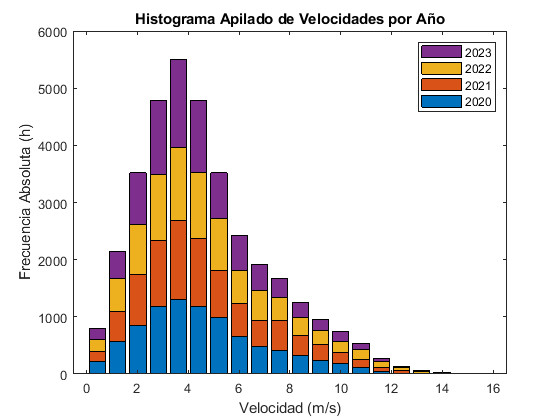
\includegraphics[width = 0.5 \textwidth]{Imagenes/Histograma Apilado de Velocidades.png}
    \caption{Histograma Apilado de Velocidades por Año.}
    \label{fig: Histograma de velocidades}
\end{figure}

En el histograma de la figura \ref{fig: Histograma de velocidades}, se observa que los valores de velocidad más frecuente se encuentran en el rango de $2$ a $6\ m/s$. Los datos correspondientes a los años 2020 y 2021 predominan en las categorías de menor velocidad, mientras que los años más recientes, 2022 y 2023, presentan una contribución más significativa en los rangos superiores.

Todos los años cuentan con una buena calidad de datos, por lo que se selecciona el año más reciente, 2023, para realizar los estudios posteriores.

\subsection{Rosa de los vientos}
% Realizar la rosa de los vientos del año seleccionado anteriormente, se valorará que se combine con frecuencia de velocidades en cada dirección (tres tramos de velocidades).

En esta subsección se presenta la rosa de los vientos para el año 2023 según tres tramos de velocidad (figura \ref{fig: Rosa de los vientos}). Observándose dos vientos predominantes en la zona: levante, con velocidades entre $5$ y $10\ m/s$  y poniente, con velocidades más bajas. Este es un comportamiento característico de las regiones costeras con influencia tanto del mar Mediterráneo como del océano Atlántico.

\begin{figure}[h]
    \centering
    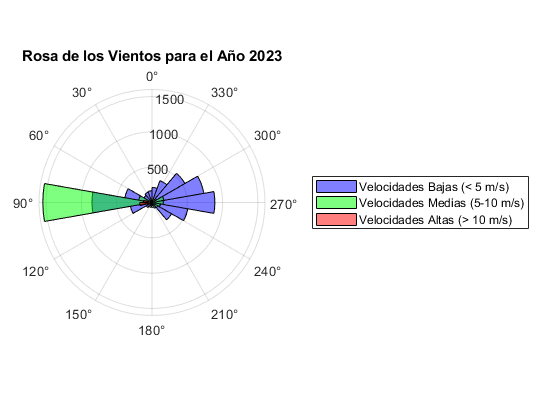
\includegraphics[width = 0.5 \textwidth]{Imagenes/Rosa de los Vientos.png}
    \caption{Rosa de los vientos.}
    \label{fig: Rosa de los vientos}
\end{figure}

\subsection{Perfil de velocidades}
% Calcular el perfil de velocidades con la altura hasta 200 m para la ubicación elegida teniendo en cuenta la oleografía del terreno. Usar la velocidad media del año seleccionado suponinedo que fue medida a 10 m.

El perfil de velocidades con la altura ($h$) se define con la ecuación:
\begin{equation}
    v(h) = v_{ref} \frac{ln \left( \frac{h}{z_0} \right)}{ln \left( \frac{h_{ref}}{z_0} \right)}
    \label{eq: Perfil de Velocidades}
\end{equation}
Donde $z_0$ es la logitud de rugosidad tabulada en la Tabla \ref{Tabla: Clase y longitud de rugosidad.} incluida en el anexo, y en este caso, sería el valor que corresponde a ``Tierra agrícola abierta sin vallas ni setos; tal vez algunos edificios separados y colinas muy suave'' con  $z_0 = 0.03$. Tomando una altura de referencia, $h_{ref} = 10\ m$, y como velocidad de referencia la velocidad media en ese año (2023), $v_{ref} = 4.5046\ m/s$. 

Aplicando la ecuación \ref{eq: Perfil de Velocidades} se obtiene el perfil de velocidades mostrado en la figura \ref{fig: Perfil de Velocidades}, alcanzando los $6.83\ m/s$ a $200\ m$ de altura.

\begin{figure}[h]
    \centering
    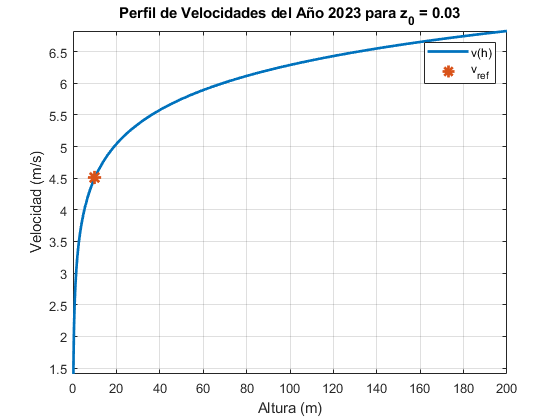
\includegraphics[width = 0.5 \textwidth]{Imagenes/Perfil de Velocidades.png}
    \caption{Perfil de Velocidades.}
    \label{fig: Perfil de Velocidades}
\end{figure}

\section{Potencia y energía del aerogenerador en la ubicación}
% A continuación, la sección de cálculo de potencia y energía donde se presentan los resultados de la densidad de energía, la energía media y factor de carga del aerogenerador. "4. Potencia y energía del aerogenerador en la ubicación".

% ----------------------------------------------------------------------------------------------

\subsection{Histograma de velocidades a la altura del buje}

% Del año representativo, obtener el histograma de velocidades teniendo en cuenta la altura del buje del aerogenerador. Representar el histograma y la frecuencia acumulada.

Teniendo una altura del buje del aerogenerador de $80\ m$, se obtiene el histograma de velocidades para el año 2023 mostrado en la figura \ref{fig: Histograma de velocidades Buje} y un histograma de frecuencia acumulada (figura \ref{fig: Histograma de velocidades Frecuencia Acumulada Buje}).

\begin{figure}[h]
    \centering
    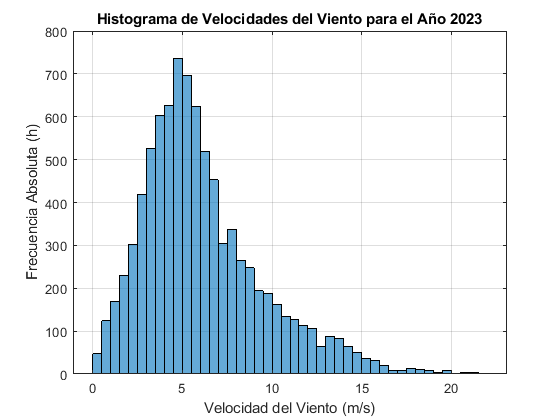
\includegraphics[width = 0.5 \textwidth]{Imagenes/Histograma de Velocidades Buje.png}
    \caption{Histograma de velocidades a la altura del buje}
    \label{fig: Histograma de velocidades Buje}
\end{figure}

\begin{figure}[h]
    \centering
    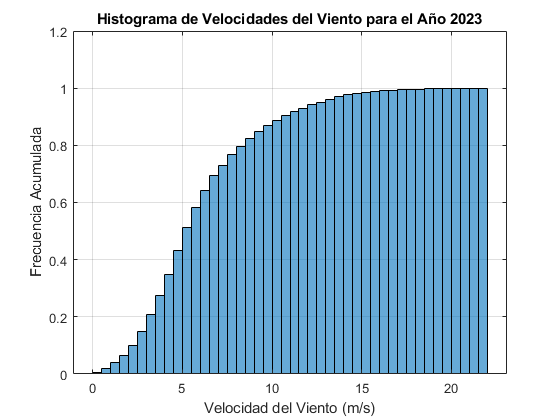
\includegraphics[width = 0.5 \textwidth]{Imagenes/Histograma de Velocidades Buje Frec Acumulada.png}
    \caption{Histograma de velocidades a la altura del buje - frecuencia acumulada}
    \label{fig: Histograma de velocidades Frecuencia Acumulada Buje}
\end{figure}

Se observa un cambio en la forma de la distribución con respecto a la figura \ref{fig: Histograma de velocidades}, debido a la extrapolación de la velocidad, en la que se multiplican las velocidades por una constante dada por la ecuación \ref{eq: Constante Velocidades Buje}.

\begin{equation}
    K = \frac{ln \left( \frac{h_{buje}}{z_0} \right)}{ln \left( \frac{h_{ref}}{z_0} \right)} = 1.358
    \label{eq: Constante Velocidades Buje}
\end{equation}

Por otro lado, el histograma de frecuencia acumulada de la figura \ref{fig: Histograma de velocidades Frecuencia Acumulada Buje}, permite identificar que aproximadamente el $50\%$ de las velocidades del viento se encuentran por debajo de los $10\ m/s$, lo que indica que la mayoría de los valores se concentran en rangos bajos a moderados. Hacia el extremo superior, se aprecia que las velocidades por encima de $20\ m/s$ son menos frecuentes. 

\subsection{Ajuste de la distribución de Weibull}
% Ajustar la distribución de Weibull al histograma de velocidades discutiendo la bondad del ajuste.

Los datos de la velocidad del viento se pueden ajustar a una distribución conocida como es la distribución de Weibull. La función de densidad de probabilidad de Weibull viene dada por la ecuación \ref{eq: Funcion de Densidad de Probabilidad de Weibull}.

\begin{equation}
    f(x) = \left\{ \frac{k}{C} \left( \frac{x}{C} \right)^{k - 1} e^{-(x/C)^k} \quad x \geq 0 \atop 0 \quad x < 0 \right.
    \label{eq: Funcion de Densidad de Probabilidad de Weibull}
\end{equation}

Asímismo, la función de probabilidad acumulada viene dada por la ecuación \ref{eq: Funcion de Probabilidad Acumulada de Weibull}.

\begin{equation}
    F(x) = \left\{ 1 - e^{-(x/C)^k} \quad x \geq 0 \atop 0 \quad x < 0 \right.
    \label{eq: Funcion de Probabilidad Acumulada de Weibull}
\end{equation}

La distribución de Weibull depende de los parámetros $k$ y $c$, que pueden estimarse mediante un ajuste de mínimos cuadrados a la distribución de datos que tenemos.

Se recomienda hacer este cálculo aplicando el siguiente cambio de variables, siendo $x_i$ las velocidades medidas y $F_i$ la frecuencia acumulada normalizada para cierto $x_i$:
\begin{gather*}
    p_i = ln(x_i) \\
    q_i = ln(- ln(1 - F_i)) \\
    u = k \\
    v = k ln(C)
\end{gather*}

Sustituyendo los cambios de variables obtenemos la ecuación lineal \ref{eq: Funcion de Probabilidad Acumulada de Weibull Cambios de Variable}

\begin{equation}
    q_i = p_i \cdot u - v
    \label{eq: Funcion de Probabilidad Acumulada de Weibull Cambios de Variable}
\end{equation}

El ajuste realizado se muestra en la figura \ref{fig: Ajuste de la distribución de Weibull}, a partir del cual se obtienen los valores $k = 2.0498$ y $C = 6.877$, con un coeficiente de determinación $R^2 = 0.9917$, lo que indica que el ajuste es bueno.

\begin{figure}[h]
    \centering
    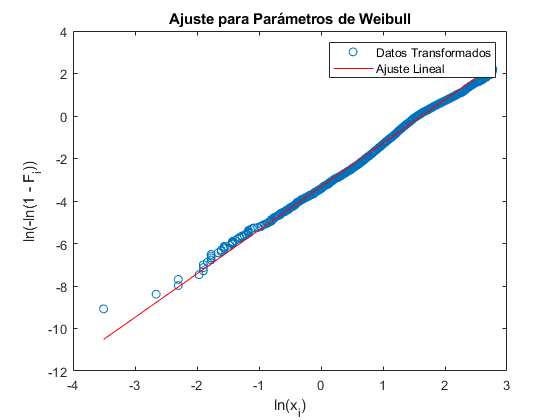
\includegraphics[width = 0.5 \textwidth]{Imagenes/Ajuste de Distribucion de Weibull.png}
    \caption{Ajuste de la distribución de Weibull.}
    \label{fig: Ajuste de la distribución de Weibull}
\end{figure}


\subsection{Curva de densidad de Weibull}
% Calcular y representar la curva de densidad de Weibull a partir de los parámetros ajustados en el rango de velocidades adecuado. Comparar el resultado con el histograma de velocidades del año representativo.

Una vez calculados los parámetros $k$ y $C$, podemos representar la curva de densidad de Weibull y compararla con el histograma de velocidades (figura \ref{fig: Curva de densidad de Weibull vs Histograma de velocidades}).

\begin{figure}[h]
    \centering
    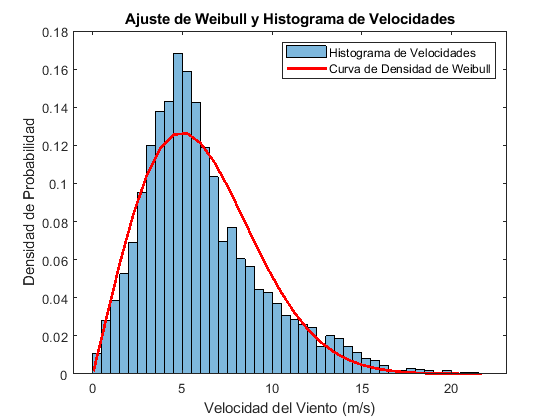
\includegraphics[width = 0.5 \textwidth]{Imagenes/Ajuste de Weibull y Histograma de Velocidades.png}
    \caption{Comparación de la curva de densidad de Weibull con el histograma de velocidades.}
    \label{fig: Curva de densidad de Weibull vs Histograma de velocidades}
\end{figure}

\subsection{Curva de energía proporcionada por el aerogenerador}
% Calcular y representar la curva de energía proporcionada por el aerogenerador para cada intervalo de velocidades, usando la función de densidad de Weibull del apartado anterior, y la curva de potencia proporcionada en la Tabla 2. Evaluar la energía anual producida, y el factor de carga. Discutir los valores.

A partir de los datos sobre la potencia del aerogenerador expuestos en la tabla \ref{Tabla: Curva de potencia} del anexo, y la curva de densidad de Weibull previamente calculada, se calcula y representa la curva de energía proporcionada por el aerogenerador en la figura \ref{fig: Curva de energia proporcionada por el aerogenerador}.

\begin{figure}[h]
    \centering
    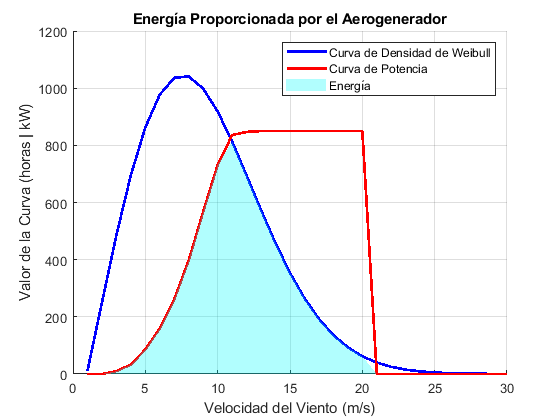
\includegraphics[width = 0.5 \textwidth]{Imagenes/Curva de Energia.png}
    \caption{Comparación de energía proporcionada por el aerogenerador.}
    \label{fig: Curva de energia proporcionada por el aerogenerador}
\end{figure}

Se obtiene que el aerogenerador proporciona una energía de $5265\ MWh$ al año, que para un aerogenerador de $850\ kW$ de potencia nominal supone un factor de carga de $0.7071$.


\section{Conclusiones}
% Por último, la sección conclusiones, "5. Conclusiones". Discusión en 2 o 3 párrafos de las conclusiones más relevantes del análisis de los datos eólicos para la ubicación elegida que han permitido el cumplimiento de los objetivos. Discusión justificada de la viabilidad de un parque eólico en la ubicación.

Tras el análisis estadístico del recurso eólico en la Isla de Tarifa y el cálculo de la energía generada por un aerogenerador de $850\ kW$ de potencia nominal, se concluye que la ubicación es altamente favorable para la instalación de un parque eólico. Los datos del año 2023 fueron ajustados a una distribución de Weibull, obteniendo un coeficiente de determinación $R^2 = 0.9917$, lo que confirma la calidad de los datos y respalda la validez del estudio.

Se obtuvo un factor de carga de $0.7071$, lo que indica que el emplazamiento es excelente para un parque eólico. Aunque en 2023 aproximadamente el $50\%$ de las velocidades registradas fueron inferiores a $10\ m/s$, se ha observado un incremento en las velocidades superiores en los últimos años, lo que sugiere un posible aumento en la generación futura de energía.

El parque eólico de Tahivilla (Tarifa), respalda esta conclusión. Dicho parque está en proceso de modernización para incrementar su capacidad de $78.4\ MW$ a $84.4\ MW$. Sin embargo, aunque el análisis técnico es favorable, la construcción de un parque eólico en la Isla de Tarifa no sería posible debido a las restricciones impuestas por la declaración del Parque Nacional del Estrecho de Gibraltar en 2003, que supone la protección de la isla y de sus aguas más inmediatas.

%\section{Bibliografía}
\printbibliography % Imprime la bibliografía

\newpage
\onecolumn

\addcontentsline{toc}{section}{Anexos}
\thispagestyle{empty}
\begin{center}
    {
\includegraphics[width=0.5\textwidth]{Imagenes/Logo UPM.png}\par}
    \vspace{1cm}
    {\bfseries\LARGE Escuela Técnica Superior de Ingenieros Industriales \par}
    \vspace{0.5cm}
    {\scshape\Large Máster en Ingeniería Industrial \par}
    \vspace{3cm}
    {\scshape\Huge Anexos \par}
    \vspace{1.5cm}
    {\itshape\Large Estudio del Recurso Eólico en Tarifa \par}
    \vfill
    {\Large Autora: Mercedes Román Ruiz \par}
    \vspace{0.5cm}
    {\Large \Fecha \par}
\end{center}

\newpage

\begin{table}[H]
    \centering
    \label{Tabla: Clase y longitud de rugosidad.}
    \caption{Clase y longitud de rugosidad para los distintos paisajes según \textit{European Wind Atlas}}
    \begin{tabular}{|l|l|p{13cm}|}
        \hline
        Clase & $z_0(m)$ & Tipo de paisaje \\
        \hline
        0 & 0.0002 & Superficies de agua: mares y lagos \\
        0.5 & 0.0024 & Terreno abierto con superficie lisa, p. hormigón, pistas de aeropuerto,hierba cortada, etc. \\
        1 & 0.03 & Tierra agrícola abierta sin valals ni setos; tal vez algunos edificios muy separados y colinas muy suave \\
        1.5 & 0.055 & Terreno agrícola con algunas edificaciones y setos de 8 m de altura separados por más de 1 km \\
        2 & 0.1 & Terreno agrícola con algunos edificios y setos de 8 m de altura separados por aprox. 500 metros \\
        2.5 & 0.2 & Terreno agrícola con muchos árboles, arbustos y plantas, o setos de 8 m de altura separados por aprox. 250 metros \\
        3 & 0.4 & Pueblos, aldeas, terrenos agrícolas con muchos o altos setos, bosques y terrenos muy accidentados y desnivelados \\
        3.5 & 0.6 & Grandes ciudades con edificios altos. \\
        4 & 1.6 & Grandes ciudades con edificios altos y rascacielos. \\ 
        \hline
    \end{tabular}
\end{table}

\begin{table}[H]
    \centering
    \label{Tabla: Curva de potencia}
    \caption{Potencia de un aerogenerador genérico con $850 kW$ de potencia nominal.}
    \begin{tabular}{|r | r|}
        \hline
        $v(m/s)$ & $P(kW)$ \\
        \hline
        1 & 0 \\
        2 & 0 \\
        3 & 10 \\ 
        4 & 33 \\
        5 & 86 \\
        6 & 160 \\
        7 & 262 \\ 
        8 & 398 \\
        9 & 568 \\
        10 & 732 \\ 
        11 & 836 \\
        12 & 847 \\
        13 & 850 \\
        14 & 850 \\
        15 & 850 \\
        16 & 850 \\
        17 & 850 \\
        18 & 850 \\
        19 & 850 \\
        20 & 850 \\
        21 & 0 \\
        22 & 0 \\
        23 & 0 \\
        24 & 0 \\
        25 & 0 \\
        26 & 0 \\
        27 & 0 \\
        28 & 0 \\
        29 & 0 \\
        30 & 0 \\
        \hline
    \end{tabular}
\end{table}

\end{document}
